\documentclass{standalone}

\usepackage{tikz}
\usetikzlibrary{shapes}
\usetikzlibrary{arrows}
\usetikzlibrary{positioning}

\begin{document}
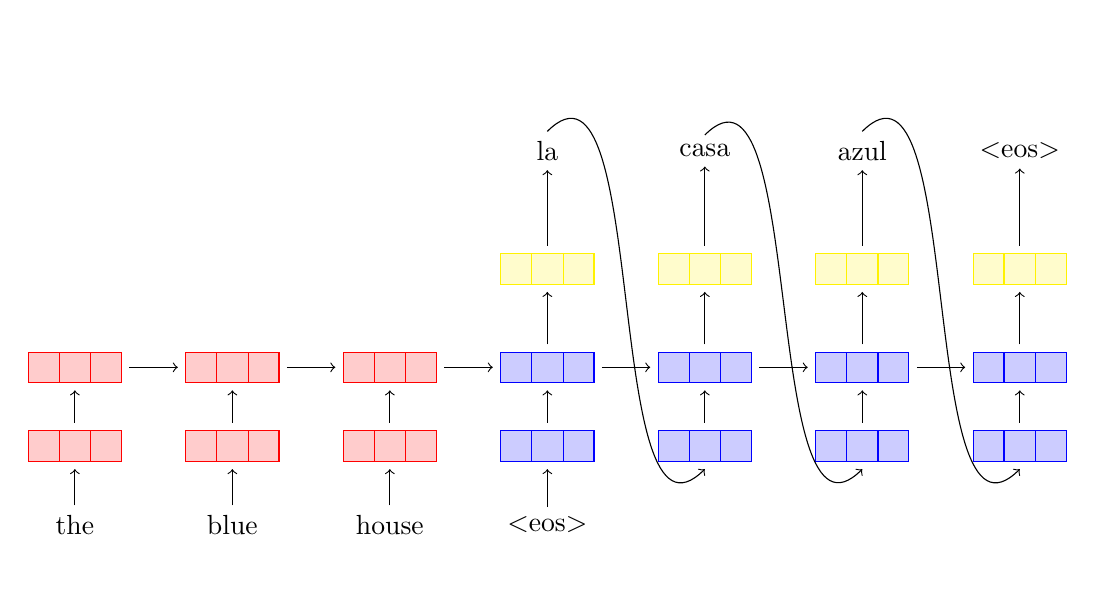
\begin{tikzpicture}[
  hid/.style 2 args={
    rectangle split,
    rectangle split horizontal,
    draw=#2,
    rectangle split parts=#1,
    fill=#2!20,
    outer sep=1mm}]
  % draw input nodes
  \foreach \i [count=\step from 1] in {the,blue,house,{{$<$eos$>$}}}
    \node (i\step) at (2*\step, -2) {\i};
  % draw output nodes
  \foreach \t [count=\step from 4] in {la,casa,azul,{{$<$eos$>$}}} {
    \node[align=center] (o\step) at (2*\step, +2.75) {\t};
  }
  % draw embedding and hidden layers for text input
  \foreach \step in {1,...,3} {
    \node[hid={3}{red}] (h\step) at (2*\step, 0) {};
    \node[hid={3}{red}] (e\step) at (2*\step, -1) {};    
    \draw[->] (i\step.north) -> (e\step.south);
    \draw[->] (e\step.north) -> (h\step.south);
  }
  % draw embedding and hidden layers for label input
  \foreach \step in {4,...,7} {
    \node[hid={3}{yellow}] (s\step) at (2*\step, 1.25) {};
    \node[hid={3}{blue}] (h\step) at (2*\step, 0) {};
    \node[hid={3}{blue}] (e\step) at (2*\step, -1) {};    
    \draw[->] (e\step.north) -> (h\step.south);
    \draw[->] (h\step.north) -> (s\step.south);
    \draw[->] (s\step.north) -> (o\step.south);
  }  
  % edge case: draw edge for special input token
  \draw[->] (i4.north) -> (e4.south);
  % draw recurrent links
  \foreach \step in {1,...,6} {
    \pgfmathtruncatemacro{\next}{add(\step,1)}
    \draw[->] (h\step.east) -> (h\next.west);
  }
  % draw predicted-labels-as-inputs links
  \foreach \step in {4,...,6} {
    \pgfmathtruncatemacro{\next}{add(\step,1)}
    \path (o\step.north) edge[->,out=45,in=225] (e\next.south);
  }
\end{tikzpicture}
\end{document}